\chapter[SCP-030 人造人]{
    SCP-030 The Homunculus\\
    SCP-030 人造人
}

\label{chap:SCP-030}

\begin{figure}[H]
    \centering
    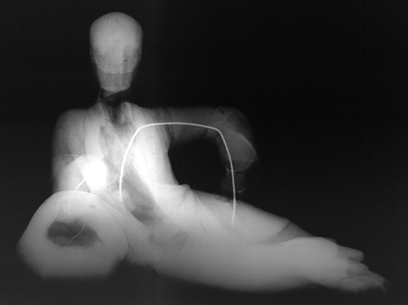
\includegraphics[width=0.5\linewidth]{images/SCP.030.jpg}
    \caption*{一张SCP-030的X光照片。从其躯干连至左臂的线状物体是其定位系统的一部分。}
\end{figure}

\bb{项目编号:}SCP-030

\bb{安全等级:}Safe

\bb{特殊收容措施:}SCP-030被收容于Site-17中一个改造过的人形生物收容室中。改造包括一些为适应其身材而作出的调整,例如合适尺寸的工作台与椅子。室内的亮度可依SCP-030的要求通过一个简单的调光器进行调整,最大可调至2000流明。如果需要使SCP-030进入惰性状态,工作人员可以通过外部开关关闭照明且在有必要时可拉上遮光窗帘。已有提供标准夜视设备以便观察惰性状态中的SCP-030。

SCP-030可能会每90天一次要求个人研究所需的材料。所有之前所要求的材料将被收集起来并在给予新材料之前销毁。所有的材料将被研究人员与安保人员进行评估与筛查。禁止SCP-030获取任何现代科学期刊或文档,且对其提供的小说写作时间不得晚于公元1623年,以确保其固有知识的完整。

希望与SCP-030进行书面交流的人员需向当前研究主管提交一份正式申请(文件\#30-RS\slash B)。所有的来往书信均会被保存。希望与SCP-030进行当面交流的人员需在交流日期的至少30天前向站点总管提交一份正式申请(文件030-RP\slash ,17-030\slash A)。所有的交流内容均会被记录并保存。资深研究员可以申请令SCP-030暂时从其收容室中离开至多一个小时,在Site-17内对未受限材料或事件提供旁观者的观点。在任何情况下SCP-030均不能离开Site-17。该申请必须在观察解禁日期的至少30天前当面提交给站点主管与安保人员。所有的观察解禁事件均会被记录并保存。SCP-030已装备有跟踪设备(设备控制码\#030-17-1),故可以在任何时候准确判断其在Site-17内的位置。

\bb{描述:}SCP-030外表为一无发,无性,灰色皮肤的人类,身高71厘米(28英尺),体重12.70千克(在旧单位中为二英石)。它的实心蓝色眼球没有可分辨的虹膜或瞳孔,看上去像切割过的小块蓝宝石。SCP-030的声线雌雄难辨,其拥有明显的英国口音,但目前无法细分至任何现代地区。它能够用古希腊语、拉丁语、意大利语、英语、西班牙语、葡萄牙语以及两(2)种目前未能分辨的语言——尽管SCP-030坚持它们应该是“常识”——进行对话与读写。SCP-030还展现出在物理、化学、天文学、数学及园艺方面与公元17世纪学院水平大致相等的知识。此外,SCP-030还在这些方面表现出了历史上未有记录的研究方向的知识。这些在自然科学方面非传统的,或完全未知的研究途径是SCP-030在交流中的用途之一。

当1.5米(5英寸)内存在亮度15流明以上的光源时,SCP-030保持活跃状态。在无光条件下,SCP-030进入惰性状态,会明显地失去意识且不表现出生命迹象。在重新暴露于光线下五至十(5-10)秒后,SCP-030会再次变得活跃,无论之前停止活动的时间长短,其均像是从一次小睡中醒来。SCP-030似乎并不像人类需要睡眠一样需要那些不活跃的时间,且表现出了希望尽可能长地保持活跃状态的欲望。

对SCP-030的活体解剖并未得出明确结论。英国肯特郡,萨利郡及大伦敦当地的粘土组成了其身体的大部分,而在所有提取到的样本中均发现了曼德拉草(\ii{Mandragora officinarum}),草木灰水,水银以及人血的痕迹。SCP-030表示,若以探知其原理为目的实行全套的探索性手术,则可能会使其无法继续存在。SCP-030被取样的部分并不会恢复,故目前暂停取样以保存其完整。虽然能够伤害SCP-030,但它似乎并不感到疼痛,只是去重塑它被损伤的那一部分结构 。值得注意的是,虽然有多种工具可以用来改变其表面,SCP-030无法直接用人类的手来重塑。SCP-030并不呼吸,没有物质需求,且不产生废物;不过它的确会不频繁地要求洗澡。

SCP-030自称为“Ariel”并频繁地要求工作人员也这样称呼它。涉及SCP-030的制造法与制造者的问题总是得到程序化的回答:“我被告知要忘记这部分信息。十分抱歉。”SCP-030每次均用同样的声调和节奏回答与其来源和创造者相关的问题。

SCP-030是于6\slash 12\slash ████在一次由待建停车场引发的对伦敦摩特雷克区的强制考古勘察中被发现。它被埋在街道下约2.7米(9英尺),并装在一个小石棺内。石棺没有任何标记,鉴于在勘察地区发现了另一坟墓,当时猜想它是一名死婴的棺材。棺材的盖子在勘察中破碎,使得SCP-030暴露在日光下。在阳光的突然照射下,SCP-030在数秒内从其惰性状态醒来并作出了一个温和的举动,即对建筑队员们说“下午好”。基金会大伦敦侦察部队的一名成员在数小时内被召至现场并在未受到阻碍的情况下将样品保管。有限的几个目击者被实行记忆删除后释放。

\bb{附件1:}

\tred{文件030-C:SCP-030的安保日志}

\tred{隐藏 文件030-C:SCP-030的安保日志}

9\slash 14\slash ████:在SCP-030上安装了定位系统。

12\slash 21\slash ████:SCP-030报告其定位系统出现故障。在六(6)小时内完成了修理工作。SCP-030主动提出帮助,但出于安全理由而被拒绝了。

3\slash 13\slash ████:SCP-030完成了一个针对未知语言Alpha(“Zephyr”)的长达18轴的讲习会,五(5)名研究者被认为已熟悉掌握。词典被上传给O5-█。

7\slash 2\slash ████:在交流时,研究者██████████不经意间说了几句有关光电技术的话。在该研究者进一步详述之前交流被中止。

8\slash 12\slash ████:SCP-030要求一份镁并称它打算点燃样品以研究其产生的光。要求被研究者否决。

11\slash 14\slash ████:事故030-1:SCP-030似乎仅使用标准盆栽土壤,姜(\ii{Zingiber officinale}),一份72克的金红石石英以及23厘米长,圈成线圈的铜线制造出了一个能够以未知方式放射出高能定向紫外线的物品\slash 设备。该设备被没收。在没有SCP-030的直接介入下尚无法复制其效果。研究者正在商讨以决定SCP-030的这条研究线路是否允许继续。据推测,SCP-030可能正在研究光电效应的非传统亦或异常的表现形式,而这是在仅获得了关于光电效应极少信息之后。所有SCP-030进行的研究暂停,其获得的材料也被没收以待再次审查。
